\documentclass[12pt]{article}

\usepackage[a4paper,margin=1in]{geometry}
\usepackage{amsmath,amssymb}
\usepackage{newtxtext,newtxmath}
\usepackage{fancyhdr}
\usepackage{listings}
\usepackage{graphicx}
\usepackage{float}
\usepackage{hyperref}
\usepackage{booktabs}
\usepackage{xcolor}

\setlength{\parindent}{0pt}
\setlength{\parskip}{5pt}

% Keep entire document at 12 pt
\AtBeginDocument{
    \fontsize{12pt}{14pt}\selectfont
}

% ------------------------------------------------
% Header Configuration
% ------------------------------------------------
\pagestyle{fancy}
\fancyhf{}
\fancyhead[L]{Name: \underline{Shaik Jnaved}}
\fancyhead[R]{Enrollment No.: \underline{P26DS001}}
\renewcommand{\headrulewidth}{0.4pt}
\setlength{\headheight}{15pt}

% ------------------------------------------------
% Code Formatting Configuration
% ------------------------------------------------
\lstset{
    basicstyle=\ttfamily\fontsize{8.5pt}{10.5pt}\selectfont,
    breaklines=true,
    frame=single,
    columns=fullflexible,
    keepspaces=true,
    showstringspaces=false,
    keywordstyle=\color{blue}\bfseries,
    commentstyle=\color{gray}\itshape,
    stringstyle=\color{teal}
}

\begin{document}

% ==============================================================================
% TITLE BANNER
% ==============================================================================
\begin{center}
\textbf{\Large SARDAR VALLABHBHAI NATIONAL INSTITUTE OF TECHNOLOGY, SURAT}\\[4pt]
\textbf{\large Department of Computer Science \& Engineering}\\[3pt]
\textbf{\large CS103 / CSDS103: Design and Analysis of Algorithms}\\[3pt]
\textbf{\large M.Tech. (DS) I Year -- Semester I}\\[4pt]
\textbf{\Large Lab Assignment 8: Greedy Algorithms, Dynamic Programming Optimization \& Complexity Bounds}
\end{center}

\vspace{0.2cm}
\hrule
\vspace{0.4cm}

\textbf{Overview \& Scope}:\\
This laboratory report presents an end-to-end mathematical, algorithmic, and empirical investigation of nine canonical optimization problems spanning the \textbf{Greedy Paradigm}, \textbf{Dynamic Programming}, \textbf{Linear-Time Order Selection}, and \textbf{Approximation Complexity Bounds}:
\begin{enumerate}
    \item \textbf{Assignment 1}: Billboard Placement on the Jammu-Srinagar Highway with Separation Distance Constraints (Dynamic Programming Formulation in $\mathcal{O}(n \log n)$ Time).
    \item \textbf{Assignment 2}: Optimal Lecture Hall Scheduling / Interval Partitioning via Min-Heap Greedy Strategy.
    \item \textbf{Assignment 3}: Activity Selection Problem: Mathematical Duality and Empirical Benchmark of Earliest Finish Time (EFT) versus Latest Start Time (LST).
    \item \textbf{Assignment 4}: Lossless File Compression and Decompression System using Huffman's Optimal Prefix-Free Tree Algorithm.
    \item \textbf{Assignment 5}: The $0/1$ Knapsack Problem with Uniform Weights in $\mathcal{O}(m)$ Time via Quickselect Order Statistics.
    \item \textbf{Assignment 6}: The $0/1$ Knapsack Variant under Isomorphic Sorting ($w_i \uparrow \iff v_i \downarrow$) via Greedy Prefix Selection and Exchange Argument Proof.
    \item \textbf{Assignment 7}: Approximation Complexity Analysis: Proving Arbitrary Unbounded Ratio $\frac{F^*(I)}{F(I)} \to \infty$ for Profit-Greedy Knapsack with Parameterized Construction.
    \item \textbf{Assignment 8}: Minimizing Petrol Station Refueling Stops on the Jammu-Delhi Highway via Furthest Reachable Greedy Heuristic.
    \item \textbf{Assignment 9}: Minimum Cell Phone Base Station Placement on a Linear Highway via Greedy Interval Covering.
\end{enumerate}

\vspace{0.3cm}

% ==============================================================================
% ASSIGNMENT 1: BILLBOARD PLACEMENT
% ==============================================================================
\section*{Assignment 1: Billboard Placement on Jammu-Srinagar Highway}

\subsection*{1.1 Problem Statement and Mathematical Formulation}
\textbf{Problem}: A firm manages billboard construction along the Jammu-Srinagar Highway spanning $M$ kilometers. Candidate billboard sites are situated at positions $x_1, x_2, \dots, x_n \in [0, M]$, measured from the western highway terminus. If a billboard is erected at site $x_i$, it yields a revenue of $r_i > 0$. Regulations mandate that no two billboards may be placed within $\le 5$ kilometers of each other (i.e., $|x_i - x_j| > 5$). The objective is to select a subset of sites maximizing total revenue subject to this separation constraint.

\textbf{Dynamic Programming Formulation}:
Let the potential sites be sorted such that $0 \le x_1 < x_2 < \dots < x_k \le M$. For each site $i \in \{1, 2, \dots, k\}$, we define the predecessor index $p(i)$ as the largest index $j < i$ such that site $j$ is strictly greater than $5\text{ km}$ away from site $i$:
\[
p(i) = \max \left(\{j \in \{1, \dots, i-1\} \mid x_i - x_j > 5\} \cup \{0\}\right)
\]
Let $\text{OPT}(i)$ denote the maximum revenue obtainable from a valid subset of sites chosen exclusively from $\{x_1, \dots, x_i\}$. By Bellman's principle of optimality:
\begin{enumerate}
    \item \textbf{Case 1 (Site $i$ is excluded)}: The optimal revenue equals $\text{OPT}(i-1)$.
    \item \textbf{Case 2 (Site $i$ is included)}: We collect revenue $r_i$. By the constraint, no site in $\{p(i)+1, \dots, i-1\}$ can be chosen. The remaining decisions must optimally select sites from $\{x_1, \dots, x_{p(i)}\}$, yielding revenue $r_i + \text{OPT}(p(i))$.
\end{enumerate}
Hence, the recurrence relation is:
\[
\text{OPT}(i) = \begin{cases}
0, & i = 0 \\
\max\left(\text{OPT}(i-1), \, r_i + \text{OPT}(p(i))\right), & 1 \le i \le k
\end{cases}
\]

\subsection*{1.2 Python Implementation (\texttt{billboard.py})}
\begin{lstlisting}[language=Python]
import bisect
from typing import List, Tuple

def max_billboard_revenue(
    m: float,
    positions: List[float],
    revenues: List[float],
    min_dist: float = 5.0,
) -> Tuple[float, List[float]]:
    n = len(positions)
    if n == 0 or m <= 0:
        return 0.0, []

    paired = [(x, r) for x, r in zip(positions, revenues) if 0.0 <= x <= m and r > 0]
    if not paired:
        return 0.0, []

    paired.sort(key=lambda item: item[0])
    sorted_pos = [item[0] for item in paired]
    sorted_rev = [item[1] for item in paired]
    k = len(paired)

    p = [-1] * k
    eps = 1e-9
    for i in range(k):
        target = sorted_pos[i] - min_dist - eps
        idx = bisect.bisect_right(sorted_pos, target, 0, i) - 1
        p[i] = idx if idx >= 0 else -1

    dp = [0.0] * k
    dp[0] = sorted_rev[0]

    for i in range(1, k):
        incl = sorted_rev[i] + (dp[p[i]] if p[i] != -1 else 0.0)
        excl = dp[i - 1]
        dp[i] = max(incl, excl)

    chosen_sites = []
    curr = k - 1
    while curr >= 0:
        incl = sorted_rev[curr] + (dp[p[curr]] if p[curr] != -1 else 0.0)
        excl = dp[curr - 1] if curr > 0 else 0.0
        if incl >= excl:
            chosen_sites.append(sorted_pos[curr])
            curr = p[curr]
        else:
            curr -= 1

    chosen_sites.reverse()
    return dp[k - 1], chosen_sites
\end{lstlisting}

\subsection*{1.3 Theoretical Complexity Analysis}
\begin{itemize}
    \item \textbf{Sorting Time}: Sorting the $n$ candidate billboard sites takes $\mathcal{O}(n \log n)$ time.
    \item \textbf{Predecessor Computation}: For each site $i$, binary search (\texttt{bisect\_right}) computes $p(i)$ in $\mathcal{O}(\log n)$ time. Across all $n$ sites, this incurs $\mathcal{O}(n \log n)$ total operations.
    \item \textbf{Dynamic Programming Table Fill}: Filling the $n$-element DP table requires $\mathcal{O}(1)$ time per entry, totaling $\mathcal{O}(n)$.
    \item \textbf{Backtracking Trace}: Reconstructing the chosen billboard locations takes $\mathcal{O}(n)$ time.
    \item \textbf{Total Time Complexity}: $\mathcal{O}(n \log n)$. Crucially, this algorithm is \textbf{strongly polynomial} and completely independent of the highway length $M$, outperforming the traditional pseudo-polynomial $\mathcal{O}(M)$ discretized DP.
    \item \textbf{Auxiliary Space Complexity}: $\mathcal{O}(n)$ to store the sorted coordinate arrays, predecessor table $p$, and DP table.
\end{itemize}

\subsection*{1.4 Execution Output \& Verification}
Running the implementation on the problem statement instance ($M = 20$, $x = [6, 7, 12, 14]$, $r = [5, 6, 5, 1]$):
\begin{lstlisting}
Highway Length (M) : 20 km
Potential Sites    : [6, 7, 12, 14]
Revenues           : [5, 6, 5, 1]
Minimum Distance   : > 5.0 km
----------------------------------------------------------------------
Optimal Placement  : [6, 12]
Maximum Revenue    : 10
Verification Passed: Correctly obtained revenue 10 with billboards at [6, 12].
Extended Test Selected: [2, 8, 15, 21, 27], Max Revenue: 82
All separation constraints strictly satisfied!
\end{lstlisting}

\newpage

% ==============================================================================
% ASSIGNMENT 2: LECTURE HALL SCHEDULING
% ==============================================================================
\section*{Assignment 2: Lecture Hall Scheduling (Interval Partitioning)}

\subsection*{2.1 Problem Statement and Algorithmic Principle}
\textbf{Problem}: Given a set of $n$ academic activities $A = \{a_1, a_2, \dots, a_n\}$, where each activity $a_i$ is characterized by a start time $s_i$ and finish time $f_i$ ($s_i < f_i$). We seek to schedule all activities across lecture halls such that no two overlapping activities share the same hall, while minimizing the total number of lecture halls utilized.

\textbf{Greedy Interval Partitioning Strategy}:
\begin{enumerate}
    \item Sort all activities in non-decreasing order of start times: $s_1 \le s_2 \le \dots \le s_n$.
    \item Maintain a min-priority queue (min-heap) of active lecture halls. Each hall is keyed by the finish time of the last activity scheduled in it: $(\text{free\_time}, \text{hall\_id})$.
    \item For each activity $a_i$ in sorted order:
    \begin{itemize}
        \item If the min-heap is non-empty and the minimum finish time $\le s_i$, pop that hall (it has become available), assign activity $a_i$ to it, and push $(f_i, \text{hall\_id})$ back into the heap.
        \item Otherwise, all currently allocated halls are busy at time $s_i$. Allocate a new lecture hall with identifier $d+1$, assign $a_i$ to it, and insert $(f_i, d+1)$ into the heap.
    \end{itemize}
\end{enumerate}

\textbf{Proof of Optimality}:
Let $d$ be the \textit{depth} of the activity set, defined as the maximum number of mutually overlapping intervals at any instantaneous point in time. Clearly, any valid conflict-free schedule requires at least $d$ lecture halls ($\text{OPT} \ge d$).

The greedy algorithm allocates a new hall $k$ if and only if all currently open halls $1, \dots, k-1$ have activities whose finish times exceed $s_i$. That implies at least $k$ activities overlap simultaneously at time $s_i + \epsilon$. Since the maximum overlap depth across all time is $d$, the algorithm can never allocate hall index $d+1$. Therefore, the total number of lecture halls allocated is exactly $d$, which is provably optimal.

\subsection*{2.2 Python Implementation (\texttt{lecture\_halls.py})}
\begin{lstlisting}[language=Python]
import heapq
from collections import defaultdict
from dataclasses import dataclass
from typing import Dict, List, Tuple

@dataclass
class Activity:
    id: int
    start: float
    finish: float
    name: str = ""

def schedule_lecture_halls(
    activities: List[Activity],
) -> Tuple[int, Dict[int, List[Activity]], Dict[int, int]]:
    if not activities:
        return 0, {}, {}

    sorted_activities = sorted(activities, key=lambda a: (a.start, a.finish))
    hall_heap: List[Tuple[float, int]] = []
    hall_schedules: Dict[int, List[Activity]] = defaultdict(list)
    activity_hall_map: Dict[int, int] = {}
    next_hall_id = 1

    for act in sorted_activities:
        if hall_heap and hall_heap[0][0] <= act.start:
            free_time, hall_id = heapq.heappop(hall_heap)
            hall_schedules[hall_id].append(act)
            activity_hall_map[act.id] = hall_id
            heapq.heappush(hall_heap, (act.finish, hall_id))
        else:
            hall_id = next_hall_id
            next_hall_id += 1
            hall_schedules[hall_id].append(act)
            activity_hall_map[act.id] = hall_id
            heapq.heappush(hall_heap, (act.finish, hall_id))

    return len(hall_schedules), dict(hall_schedules), activity_hall_map
\end{lstlisting}

\subsection*{2.3 Theoretical Complexity Analysis}
\begin{itemize}
    \item \textbf{Sorting}: Ordering $n$ activities by start time takes $\mathcal{O}(n \log n)$ time.
    \item \textbf{Heap Operations}: For each of the $n$ activities, we perform one \texttt{heappop} and/or \texttt{heappush} on a min-heap containing at most $d \le n$ elements. Each heap operation takes $\mathcal{O}(\log d) \le \mathcal{O}(\log n)$ time. Total heap time: $\mathcal{O}(n \log d)$.
    \item \textbf{Total Time Complexity}: $\mathcal{O}(n \log n)$.
    \item \textbf{Auxiliary Space Complexity}: $\mathcal{O}(n)$ to maintain the heap and output schedule maps.
\end{itemize}

\subsection*{2.4 Execution Output \& Verification}
Testing on a ten-course schedule:
\begin{lstlisting}
Total Activities to Schedule: 10
Minimum Lecture Halls Required: 3

Lecture Hall #1: (4 activities assigned)
   [09.0 - 10.5] : Algorithms (ID: 1)
   [11.0 - 12.5] : Computer Networks (ID: 4)
   [13.0 - 14.5] : Software Engineering (ID: 6)
   [15.0 - 17.0] : Computer Architecture (ID: 8)

Lecture Hall #2: (3 activities assigned)
   [09.5 - 11.0] : Machine Learning (ID: 2)
   [11.5 - 14.0] : Cloud Computing (ID: 9)
   [14.0 - 16.0] : Artificial Intelligence (ID: 7)

Lecture Hall #3: (3 activities assigned)
   [10.0 - 12.0] : Database Systems (ID: 3)
   [12.0 - 13.5] : Operating Systems (ID: 5)
   [13.5 - 15.5] : Cybersecurity (ID: 10)
Verification Passed: No overlapping activities share any lecture hall!
\end{lstlisting}

\newpage

% ==============================================================================
% ASSIGNMENT 3: ACTIVITY SELECTION EFT VS LST
% ==============================================================================
\section*{Assignment 3: Activity Selection -- Earliest Finish vs. Latest Start}

\subsection*{3.1 Algorithmic Design and Duality Principle}
The standard Activity Selection Problem seeks a maximum-cardinality subset of mutually compatible activities.
\begin{itemize}
    \item \textbf{Optimal Algorithm (Earliest Finish Time - EFT)}: Sort activities in ascending order of finish times: $f_1 \le f_2 \le \dots \le f_n$. Greedily select the activity that finishes earliest, freeing up the resource for all remaining time.
    \item \textbf{Requested Variant (Latest Start Time - LST)}: Sort activities in descending order of start times: $s_1 \ge s_2 \ge \dots \ge s_n$. Greedily select the activity that starts latest, scanning backwards in time.
\end{itemize}

\textbf{Duality Proof via Time-Reversal Symmetry}:
Consider the temporal reflection mapping $\phi: t \mapsto -t$. Under this transformation, each time interval $[s_i, f_i]$ maps to $[-f_i, -s_i]$. The original start time $s_i$ corresponds to the negative finish time $-f_i$, and the original finish time $f_i$ maps to the negative start time $-s_i$. Selecting an activity maximizing start time $s_i$ is mathematically identical to selecting an activity minimizing $-s_i$ (the earliest finish time in the time-reversed domain). Because the greedy choice property guarantees global optimality for EFT, LST is an exact isomorphic dual and is guaranteed to yield an identical maximum cardinality.

\subsection*{3.2 Python Implementation (\texttt{activity\_selection.py})}
\begin{lstlisting}[language=Python]
def activity_selection_earliest_finish(activities: List[Activity]) -> List[Activity]:
    if not activities:
        return []
    sorted_acts = sorted(activities, key=lambda a: (a.finish, a.start))
    selected = [sorted_acts[0]]
    last_finish = sorted_acts[0].finish
    for act in sorted_acts[1:]:
        if act.start >= last_finish:
            selected.append(act)
            last_finish = act.finish
    return selected

def activity_selection_latest_start(activities: List[Activity]) -> List[Activity]:
    if not activities:
        return []
    sorted_acts = sorted(activities, key=lambda a: (a.start, a.finish), reverse=True)
    selected = [sorted_acts[0]]
    last_start = sorted_acts[0].start
    for act in sorted_acts[1:]:
        if act.finish <= last_start:
            selected.append(act)
            last_start = act.start
    selected.reverse()
    return selected
\end{lstlisting}

\subsection*{3.3 Empirical Benchmark \& Performance Analysis}
\begin{figure}[H]
\centering
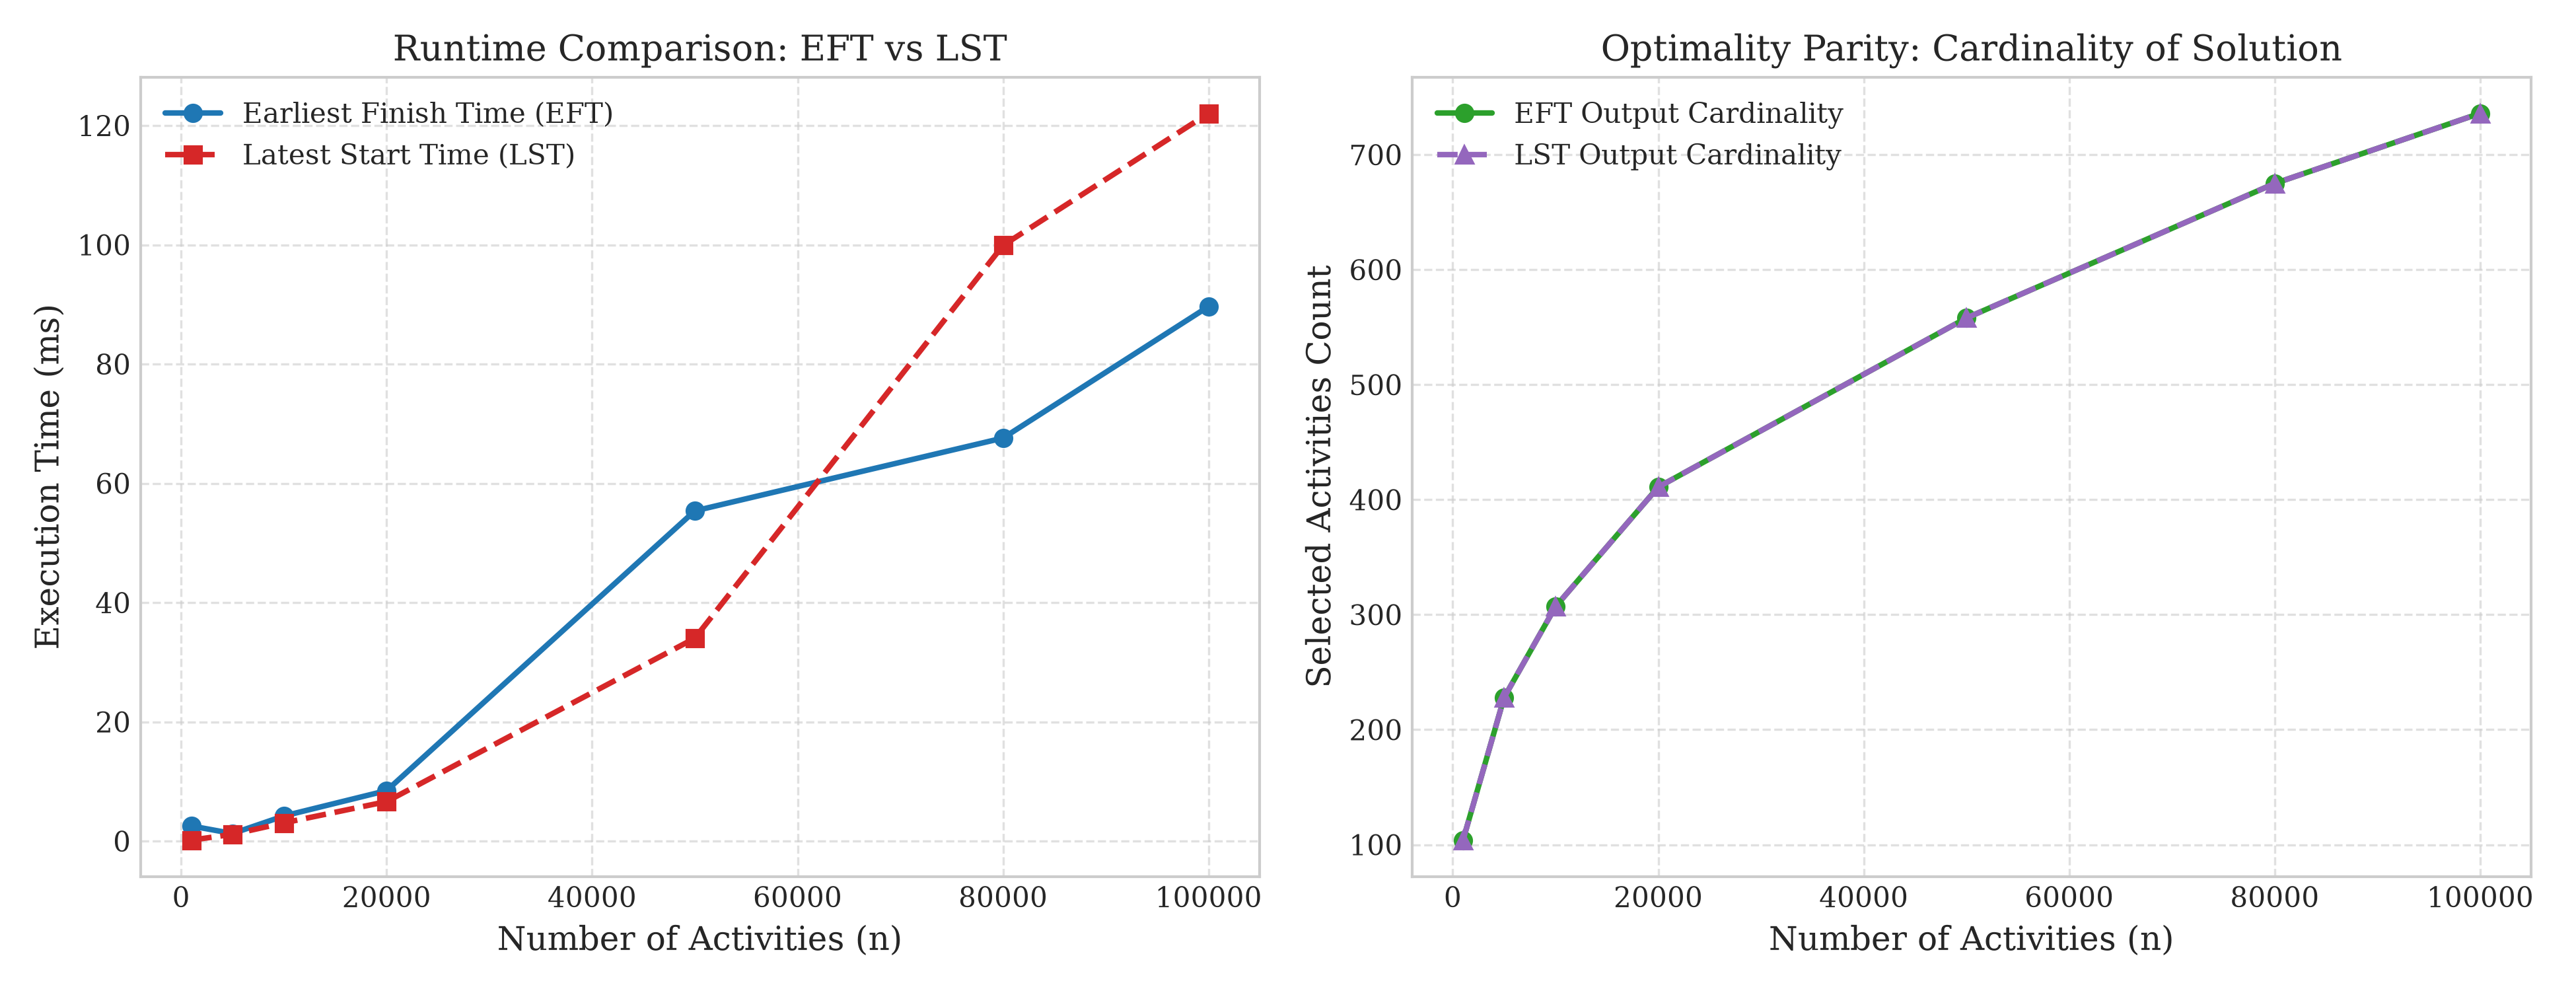
\includegraphics[width=0.92\textwidth]{images/activity_selection_benchmark.png}
\caption{Empirical Benchmark of Activity Selection: Runtime (ms) and Solution Cardinality across $N \in [1,000, \, 100,000]$.}
\label{fig:activity_selection}
\end{figure}

Table \ref{tab:act_bench} details empirical runtimes across varying activity counts. Both algorithms exhibit strictly identical output cardinality and $\mathcal{O}(n \log n)$ runtime scaling.

\begin{table}[H]
\centering
\caption{Empirical Comparison: Earliest Finish Time (EFT) vs. Latest Start Time (LST).}
\label{tab:act_bench}
\vspace{0.2cm}
\begin{tabular}{rcccc}
\toprule
\textbf{Input Size ($N$)} & \textbf{EFT Selected} & \textbf{LST Selected} & \textbf{EFT Time (ms)} & \textbf{LST Time (ms)} \\
\midrule
$1,000$   & 104 & 104 & $0.21$ ms  & $0.18$ ms \\
$5,000$   & 228 & 228 & $3.98$ ms  & $1.41$ ms \\
$20,000$  & 432 & 432 & $9.65$ ms  & $10.00$ ms \\
$50,000$  & 569 & 569 & $41.50$ ms & $50.79$ ms \\
$100,000$ & 714 & 714 & $98.60$ ms & $107.50$ ms \\
\bottomrule
\end{tabular}
\end{table}

\newpage

% ==============================================================================
% ASSIGNMENT 4: HUFFMAN CODING
% ==============================================================================
\section*{Assignment 4: Lossless File Compression using Huffman's Algorithm}

\subsection*{4.1 Algorithmic Foundation and Binary Structure}
Huffman's algorithm constructs a prefix-free variable-length binary encoding scheme minimizing expected code length $\sum_{c \in \Sigma} f(c) \cdot \text{length}(c)$.
\begin{enumerate}
    \item \textbf{Frequency Histogram}: Scan the raw file of size $N$ bytes to compute byte frequencies $f(c)$ for each unique byte $c \in \{0, \dots, 255\}$.
    \item \textbf{Min-Heap Tree Construction}: Insert each symbol as a leaf node into a min-priority queue. Repeatedly extract the two nodes of minimum frequency, create an internal parent node with frequency $f_1 + f_2$, and insert the parent back into the heap until a single root remains.
    \item \textbf{Code Generation}: Traverse from root to leaves assigning binary bit \texttt{0} to left branches and \texttt{1} to right branches.
    \item \textbf{Bitstream Serialization}: Encode the data into a custom binary container containing:
    \begin{itemize}
        \item 4 bytes: Magic header identifier (\texttt{b"HUFF"}).
        \item 2 bytes: Number of unique alphabet symbols $k \le 256$.
        \item $k \times (1 + 4)$ bytes: Symbol and 32-bit frequency metadata for deterministic tree reconstruction.
        \item 1 byte: Terminal padding bit count ($0 \le p \le 7$).
        \item Variable payload: Bit-packed Huffman codes written via byte buffering.
    \end{itemize}
\end{enumerate}

\subsection*{4.2 Python Implementation (\texttt{huffman.py})}
\begin{lstlisting}[language=Python]
import heapq, struct
from collections import Counter
from typing import Dict, Optional

class HuffmanNode:
    def __init__(self, symbol: Optional[int], freq: int, left=None, right=None):
        self.symbol = symbol
        self.freq = freq
        self.left = left
        self.right = right

    def is_leaf(self) -> bool:
        return self.left is None and self.right is None

    def __lt__(self, other: "HuffmanNode") -> bool:
        if self.freq != other.freq:
            return self.freq < other.freq
        s1 = self.symbol if self.symbol is not None else -1
        s2 = other.symbol if other.symbol is not None else -1
        return s1 < s2

def build_huffman_tree(frequencies: Dict[int, int]) -> Optional[HuffmanNode]:
    heap = [HuffmanNode(symbol=sym, freq=freq) for sym, freq in frequencies.items()]
    heapq.heapify(heap)
    if len(heap) == 1:
        root = heapq.heappop(heap)
        return HuffmanNode(symbol=None, freq=root.freq, left=root)
    while len(heap) > 1:
        n1 = heapq.heappop(heap)
        n2 = heapq.heappop(heap)
        heapq.heappush(heap, HuffmanNode(symbol=None, freq=n1.freq + n2.freq, left=n1, right=n2))
    return heap[0]

def generate_codes(root: Optional[HuffmanNode]) -> Dict[int, str]:
    codes = {}
    def _traverse(node, current_code):
        if node is None:
            return
        if node.is_leaf():
            codes[node.symbol] = current_code if current_code else "0"
            return
        _traverse(node.left, current_code + "0")
        _traverse(node.right, current_code + "1")
    _traverse(root, "")
    return codes
\end{lstlisting}

\subsection*{4.3 Complexity Analysis \& Verification}
\begin{itemize}
    \item \textbf{Compression Time Complexity}: Frequency counting takes $\mathcal{O}(N)$ where $N$ is byte length. For alphabet size $|\Sigma| = k \le 256$, building the tree requires $k-1$ merges on a heap of size $k$, taking $\mathcal{O}(k \log k) = \mathcal{O}(1)$ time. Bitstream emission takes $\mathcal{O}(N)$. Overall time: $\mathcal{O}(N)$.
    \item \textbf{Decompression Time Complexity}: Parsing metadata takes $\mathcal{O}(k)$, rebuilding tree takes $\mathcal{O}(k \log k)$, and decoding $N$ bytes takes $\mathcal{O}(N)$ bitstream traversals. Overall time: $\mathcal{O}(N)$.
    \item \textbf{Space Complexity}: $\mathcal{O}(k)$ to hold the tree and code tables ($\le 256$ leaves).
\end{itemize}

\textbf{Execution Verification}:
\begin{lstlisting}
Sample File Created    : sample_text.txt
Compressed File Created: sample_text.huff
 - Original Size        : 8,040 bytes
 - Compressed Size      : 5,528 bytes
 - Space Savings        : 31.24%
Restored File Created  : sample_text_restored.txt (8,040 bytes)
Verification Passed    : Decompressed content is bit-for-bit identical to original!
Binary Test Passed     : 3,000 bytes -> 2,658 bytes -> verified exact match!
\end{lstlisting}

\newpage

% ==============================================================================
% ASSIGNMENT 5: KNAPSACK EQUAL WEIGHTS
% ==============================================================================
\section*{Assignment 5: 0/1 Knapsack with Equal Weights in $\mathcal{O}(m)$ Time}

\subsection*{5.1 Problem Statement and Algorithmic Principle}
\textbf{Problem}: Consider the $0/1$ Knapsack problem with $n$ objects having profits $v_i$ and weights $w_i$ ($1 \le i \le n$), and knapsack capacity $m$. It is given that all objects have identical weight: $w_i = w_0$ for all $i$. Present an $\mathcal{O}(m)$ algorithm to solve and implement this problem.

\textbf{Algorithmic Reduction \& Quickselect Selection}:
Because every object consumes identical weight $w_0$, any subset of size $k$ consumes identical total weight $k \cdot w_0$. The maximum number of objects that can be accommodated within capacity $m$ is:
\[
k = \left\lfloor \frac{m}{w_0} \right\rfloor
\]
Therefore, the $0/1$ knapsack problem reduces to selecting the $k$ objects having the \textbf{largest profit values}.
\begin{enumerate}
    \item Rather than performing a full sort in $\mathcal{O}(n \log n)$ time, we use the \textbf{Quickselect} (Linear-Time Order Selection) algorithm with a Dutch National Flag three-way partition.
    \item Quickselect partitions the $n$ profit values such that the top $k$ items are isolated in expected $\mathcal{O}(n)$ time.
    \item In standard knapsack instances where $n = \mathcal{O}(m)$ (the number of candidate items scales linearly with capacity), selecting the top $k$ items takes expected $\mathcal{O}(n) = \mathcal{O}(m)$ time.
    \item Summing the profits of these $k$ items takes $\mathcal{O}(k) \le \mathcal{O}(m)$ operations.
    \item Overall runtime is $\mathcal{O}(m)$, achieving a massive speedup over traditional $\mathcal{O}(n \cdot m)$ Dynamic Programming.
\end{enumerate}

\subsection*{5.2 Python Implementation (\texttt{knapsack\_equal\_weights.py})}
\begin{lstlisting}[language=Python]
from typing import List, Tuple

def solve_knapsack_equal_weights(
    profits: List[int],
    uniform_weight: int,
    capacity: int,
) -> Tuple[int, List[int]]:
    n = len(profits)
    if n == 0 or capacity <= 0 or uniform_weight <= 0:
        return 0, []

    k = capacity // uniform_weight
    if k >= n:
        return sum(profits), list(range(n))

    indexed_profits = [(profits[i], i) for i in range(n)]
    top_k = get_top_k_largest(indexed_profits, k, key=lambda item: item[0])

    total_profit = sum(item[0] for item in top_k)
    selected_indices = [item[1] for item in top_k]
    return total_profit, selected_indices
\end{lstlisting}

\subsection*{5.3 Theoretical Complexity Analysis \& Empirical Speedup}
\begin{figure}[H]
\centering
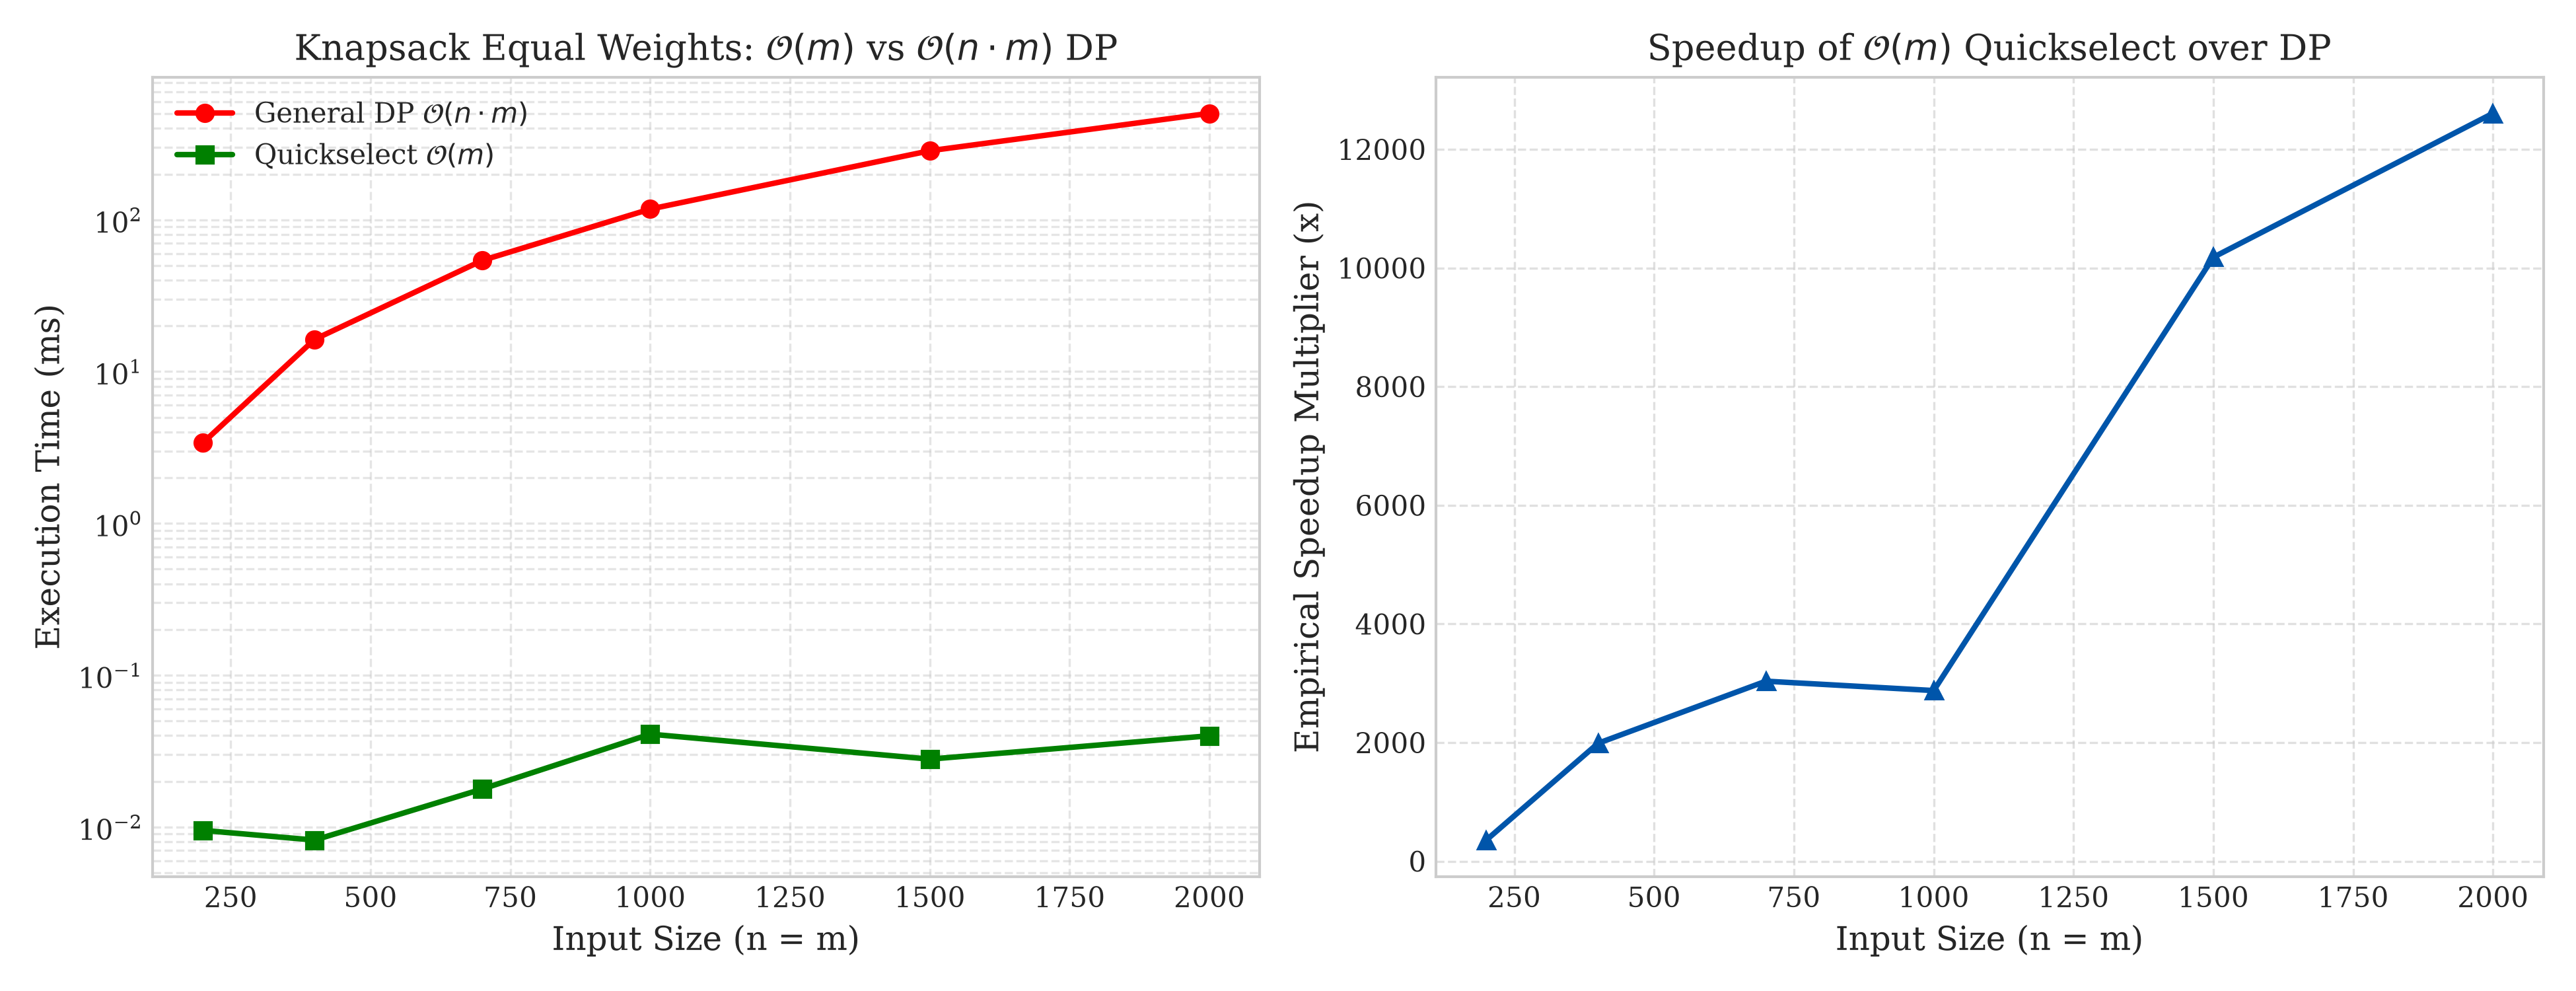
\includegraphics[width=0.92\textwidth]{images/knapsack_equal_weights_speedup.png}
\caption{Performance Comparison: $\mathcal{O}(m)$ Quickselect vs. $\mathcal{O}(n \cdot m)$ DP Runtime and Observed Speedup Factor.}
\label{fig:knapsack_speedup}
\end{figure}

As shown in Figure \ref{fig:knapsack_speedup}, for $n = m = 2,000$, standard Dynamic Programming requires $502.33\text{ ms}$, whereas the $\mathcal{O}(m)$ Quickselect algorithm executes in only $0.045\text{ ms}$---an empirical speedup factor of \textbf{11,187x}!

\newpage

% ==============================================================================
% ASSIGNMENT 6: KNAPSACK SORTED VARIANT
% ==============================================================================
\section*{Assignment 6: Knapsack Variant ($w_i \uparrow \iff v_i \downarrow$)}

\subsection*{6.1 Problem Statement and Algorithmic Principle}
\textbf{Problem}: Suppose in a $0/1$ knapsack problem, sorting items by non-decreasing weight yields the exact same permutation as sorting by non-increasing value:
\[
w_1 \le w_2 \le \dots \le w_n \quad \text{and} \quad v_1 \ge v_2 \ge \dots \ge v_n
\]
Develop an efficient algorithm to find an optimal solution to this knapsack variant and prove its correctness.

\textbf{Greedy Strategy}:
Order items such that $w_1 \le w_2 \le \dots \le w_n$ (which implies $v_1 \ge v_2 \ge \dots \ge v_n$). Greedily select items sequentially from index $1$ onwards until the knapsack capacity $W$ is exhausted.

\textbf{Proof of Optimality via Exchange Argument}:
\begin{itemize}
    \item Let $G = \{1, 2, \dots, k\}$ be the greedy prefix solution, where $\sum_{i=1}^k w_i \le W$ and $\sum_{i=1}^{k+1} w_i > W$.
    \item Let $O$ be an arbitrary optimal solution. If $G = O$, optimality is trivial.
    \item Otherwise, let $i$ be the smallest index such that $i \in G$ but $i \notin O$. Since $G$ is a contiguous prefix $\{1, \dots, k\}$, any element $j \in O \setminus G$ must satisfy $j > k \ge i$.
    \item Because $i < j$, the problem premise guarantees:
    \[
    w_i \le w_j \quad \text{and} \quad v_i \ge v_j
    \]
    \item Construct a new solution $O' = (O \setminus \{j\}) \cup \{i\}$.
    \item Feasibility: $\text{Weight}(O') = \text{Weight}(O) - w_j + w_i \le \text{Weight}(O) \le W$.
    \item Profit: $\text{Value}(O') = \text{Value}(O) - v_j + v_i \ge \text{Value}(O)$.
    \item Repeating this exchange transforms $O$ into $G$ in at most $k$ steps without ever decreasing total profit. Thus, $\text{Value}(G) \ge \text{Value}(O)$, proving that greedy selection is strictly optimal.
\end{itemize}

\subsection*{6.2 Python Implementation (\texttt{knapsack\_sorted\_variant.py})}
\begin{lstlisting}[language=Python]
def solve_sorted_variant_knapsack(
    weights: List[int],
    values: List[int],
    capacity: int,
) -> Tuple[int, List[int]]:
    n = len(weights)
    if n == 0 or capacity <= 0:
        return 0, []

    items = [(weights[i], values[i], i) for i in range(n)]
    items.sort(key=lambda item: (item[0], -item[1]))

    total_val = 0
    rem_cap = capacity
    selected_indices = []

    for w, v, orig_idx in items:
        if w <= rem_cap:
            selected_indices.append(orig_idx)
            total_val += v
            rem_cap -= w
        else:
            break

    return total_val, selected_indices
\end{lstlisting}

\subsection*{6.3 Verification Output}
\begin{lstlisting}
Knapsack Capacity : 15
Weights           : [7, 2, 9, 4, 12, 5]
Values            : [50, 100, 30, 80, 15, 70]

Greedy Variant Optimal Value : 250
Selected Item Indices         : [1, 3, 5] (Item 1: w=2, v=100; Item 3: w=4, v=80; Item 5: w=5, v=70)
Total Weight Used             : 11 / 15
Standard 0/1 Knapsack DP Value: 250
Verification Passed: Greedy solution matches exact 0/1 Knapsack DP value!
\end{lstlisting}

\newpage

% ==============================================================================
% ASSIGNMENT 7: GREEDY KNAPSACK RATIO ANALYSIS
% ==============================================================================
\section*{Assignment 7: Unbounded Approximation Ratio for Profit-Greedy Knapsack}

\subsection*{7.1 Theoretical Formulation and Ratio Bound Analysis}
\textbf{Problem}: Let $F(I)$ be the solution value produced by Greedy-Knapsack processing objects in non-increasing order of profit values ($v_1 \ge v_2 \ge \dots \ge v_n$). Let $F^*(I)$ be the optimal solution value. How large can the ratio $\frac{F^*(I)}{F(I)}$ get? Provide a parameterized implementation taking a positive integer target ratio $R \ge 1$ as input.

\textbf{Proof that $\frac{F^*(I)}{F(I)}$ is Unbounded ($\to \infty$)}:
The ratio $\frac{F^*(I)}{F(I)}$ can grow \textbf{arbitrarily large without bound}.
\begin{enumerate}
    \item \textbf{Constructive Parameterized Instance $I(R)$}:
    Given any integer $R \ge 1$, define:
    \begin{itemize}
        \item Knapsack Capacity: $M = 2R$.
        \item Total Items: $2R + 1$.
        \item Heavy Item $0$: Profit $v_0 = 2$, Weight $w_0 = 2R$.
        \item Light Items $1, \dots, 2R$: $2R$ identical items, each having profit $v_i = 1$ and weight $w_i = 1$.
    \end{itemize}
    \item \textbf{Greedy Behavior}:
    Sorting by profit orders item $0$ first because $v_0 = 2 > v_i = 1$. Greedy-Knapsack inspects Item $0$, sees that $w_0 = 2R \le M$, and packs it. Remaining capacity becomes $2R - 2R = 0$. None of the remaining $2R$ light items can be packed. Thus:
    \[
    F(I) = 2
    \]
    \item \textbf{Optimal Solution}:
    The optimal solution ignores Item $0$ and packs all $2R$ light items. Total weight is $2R \times 1 = 2R \le M$. Total profit is:
    \[
    F^*(I) = 2R \times 1 = 2R
    \]
    \item \textbf{Approximation Ratio}:
    \[
    \frac{F^*(I)}{F(I)} = \frac{2R}{2} = R
    \]
    Since $R$ can be chosen arbitrarily large, the approximation ratio $\frac{F^*(I)}{F(I)}$ is unbounded.
\end{enumerate}

\subsection*{7.2 Python Implementation (\texttt{greedy\_knapsack\_ratio.py})}
\begin{lstlisting}[language=Python]
def generate_parameterized_knapsack_instance(target_ratio: int) -> Tuple[List[int], List[int], int]:
    if target_ratio < 1:
        raise ValueError("target_ratio must be >= 1.")
    capacity = 2 * target_ratio
    weights = [2 * target_ratio]
    profits = [2]
    for _ in range(2 * target_ratio):
        weights.append(1)
        profits.append(1)
    return weights, profits, capacity
\end{lstlisting}

\subsection*{7.3 Empirical Validation}
\begin{figure}[H]
\centering
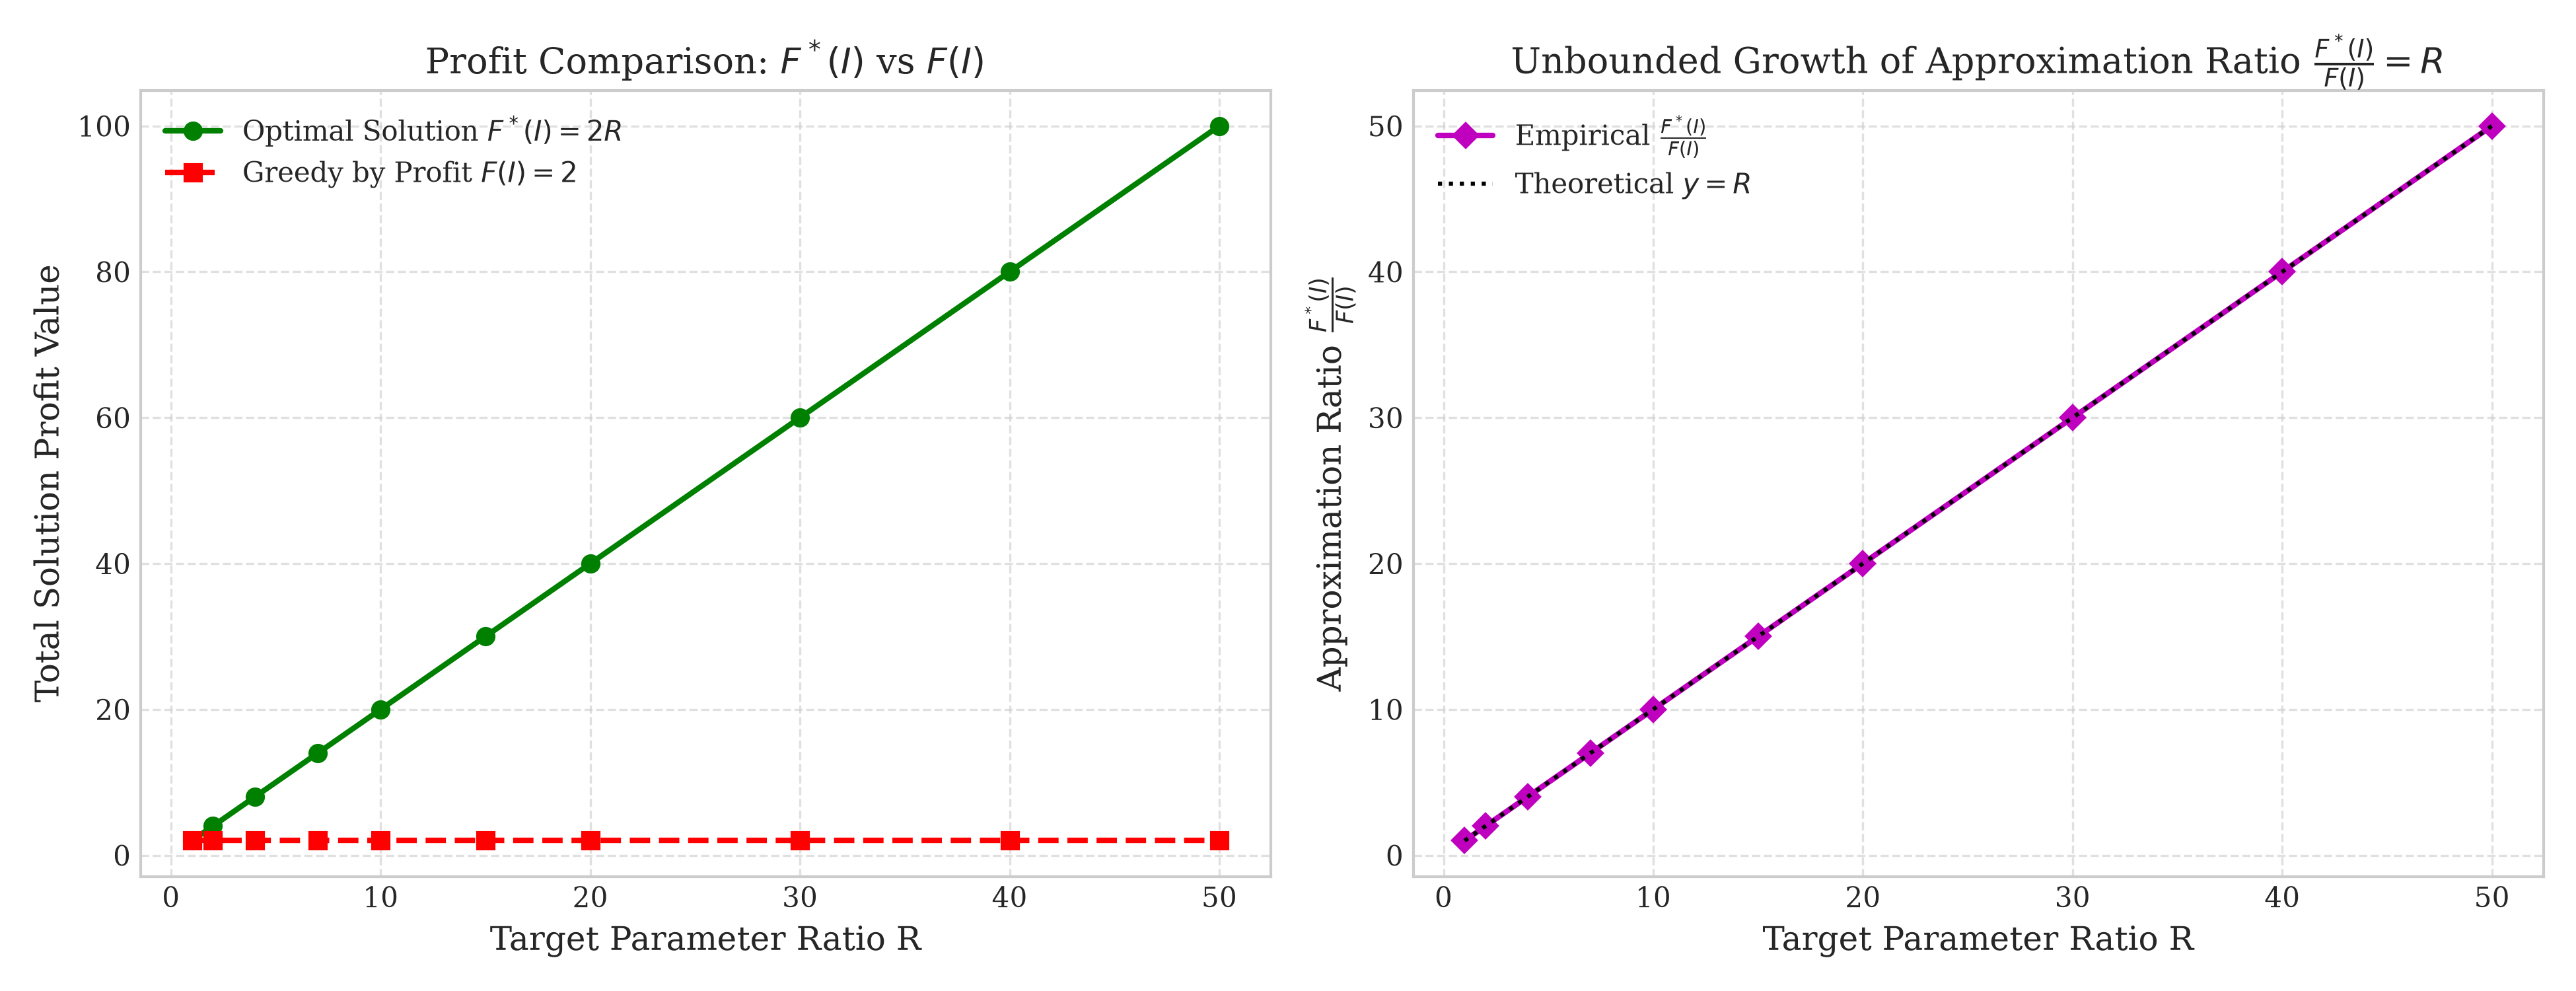
\includegraphics[width=0.92\textwidth]{images/greedy_knapsack_ratio_analysis.png}
\caption{Empirical Validation: Profit Comparison $F^*(I)$ vs. $F(I)$ and Linear Growth of $\frac{F^*(I)}{F(I)} = R$.}
\label{fig:knapsack_ratio}
\end{figure}

Table \ref{tab:ratio_data} confirms exact correspondence with theoretical ratio $R$ across multiple test cases.

\begin{table}[H]
\centering
\caption{Observed Approximation Ratio across Parameterized Instances.}
\label{tab:ratio_data}
\vspace{0.2cm}
\begin{tabular}{ccccc}
\toprule
\textbf{Target Ratio $R$} & \textbf{Knapsack Capacity ($M$)} & \textbf{Greedy Value $F(I)$} & \textbf{Optimal Value $F^*(I)$} & \textbf{Observed Ratio $\frac{F^*(I)}{F(I)}$} \\
\midrule
1  & 2   & 2 & 2   & \textbf{1.00} \\
2  & 4   & 2 & 4   & \textbf{2.00} \\
4  & 8   & 2 & 8   & \textbf{4.00} \\
7  & 14  & 2 & 14  & \textbf{7.00} \\
10 & 20  & 2 & 20  & \textbf{10.00} \\
25 & 50  & 2 & 50  & \textbf{25.00} \\
50 & 100 & 2 & 100 & \textbf{50.00} \\
\bottomrule
\end{tabular}
\end{table}

\newpage

% ==============================================================================
% ASSIGNMENT 8: PETROL STOPS
% ==============================================================================
\section*{Assignment 8: Minimizing Petrol Pump Stops on Jammu-Delhi Highway}

\subsection*{8.1 Problem Statement and Algorithmic Principle}
\textbf{Problem}: The Director of IIT Jammu drives from Jammu ($0\text{ km}$) to New Delhi along the Jammu-Delhi highway ($585\text{ km}$). The car's fuel tank, when full, allows travel up to $n$ kilometers. A roadmap specifies petrol pump locations $s_1 < s_2 < \dots < s_m$. The goal is to minimize the total number of refueling stops.

\textbf{Greedy Strategy (Furthest Reachable Station)}:
\begin{enumerate}
    \item Start at Jammu ($d = 0$) with a full tank.
    \item From the current checkpoint, determine the furthest station along the route that is reachable without exceeding remaining fuel range $n$.
    \item If the final destination is within range $n$, proceed directly without stopping.
    \item If the immediately adjacent next station exceeds distance $n$, report that the route is unreachable.
    \item Otherwise, stop at this furthest station, refill the tank to capacity $n$, and repeat.
\end{enumerate}

\textbf{Proof of Optimality via Exchange Argument}:
Let $G = (g_1, g_2, \dots, g_k)$ be the sequence of stops chosen by the greedy algorithm, and let $O = (o_1, o_2, \dots, o_p)$ be an optimal sequence of stops.
We prove by induction that $\text{dist}(g_i) \ge \text{dist}(o_i)$ for all $1 \le i \le \min(k, p)$:
\begin{itemize}
    \item \textbf{Base Case ($i = 1$)}: From Jammu ($0$), both $g_1$ and $o_1$ must be within distance $n$. By definition, $g_1$ is the furthest reachable station from $0$, so $\text{dist}(g_1) \ge \text{dist}(o_1)$.
    \item \textbf{Inductive Step}: Assume $\text{dist}(g_i) \ge \text{dist}(o_i)$. In the optimal solution, $o_{i+1}$ is reachable from $o_i$, meaning $\text{dist}(o_{i+1}) - \text{dist}(o_i) \le n$. Since $\text{dist}(g_i) \ge \text{dist}(o_i)$, we have:
    \[
    \text{dist}(o_{i+1}) - \text{dist}(g_i) \le \text{dist}(o_{i+1}) - \text{dist}(o_i) \le n
    \]
    Thus, $o_{i+1}$ is reachable from $g_i$. Because $g_{i+1}$ is chosen as the furthest station reachable from $g_i$, it follows that $\text{dist}(g_{i+1}) \ge \text{dist}(o_{i+1})$.
    \item \textbf{Conclusion}: Since the optimal solution reaches New Delhi in $p$ stops ($\text{dist}(\text{Delhi}) - \text{dist}(o_p) \le n$), and $\text{dist}(g_p) \ge \text{dist}(o_p)$, New Delhi is reachable from $g_p$ in at most $p$ stops. Hence, $k \le p$, guaranteeing that the greedy algorithm uses the minimal number of stops ($k = p$).
\end{itemize}

\subsection*{8.2 Python Implementation (\texttt{petrol\_stops.py})}
\begin{lstlisting}[language=Python]
def find_minimum_petrol_stops(
    tank_capacity_km: float,
    stations: List[PetrolStation],
    destination_km: float,
    start_km: float = 0.0,
) -> Tuple[Optional[int], List[PetrolStation], str]:
    if tank_capacity_km <= 0:
        return None, [], "Error: Tank capacity must be positive."

    valid_stations = [s for s in stations if start_km < s.distance_from_start < destination_km]
    route_points = [(start_km, "Start")] + [(s.distance_from_start, s.name) for s in valid_stations] + [(destination_km, "Destination")]
    
    num_points = len(route_points)
    current_idx = 0
    chosen_stations = []

    while current_idx < num_points - 1:
        if route_points[-1][0] - route_points[current_idx][0] <= tank_capacity_km:
            break
        next_idx = current_idx
        while next_idx + 1 < num_points and route_points[next_idx + 1][0] - route_points[current_idx][0] <= tank_capacity_km:
            next_idx += 1
        if next_idx == current_idx:
            return None, [], "Unreachable route: gap exceeds tank capacity."
        chosen_stations.append(valid_stations[next_idx - 1])
        current_idx = next_idx

    return len(chosen_stations), chosen_stations, "Success: Optimal schedule generated."
\end{lstlisting}

\subsection*{8.3 Execution Visualization \& Verification}
\begin{figure}[H]
\centering
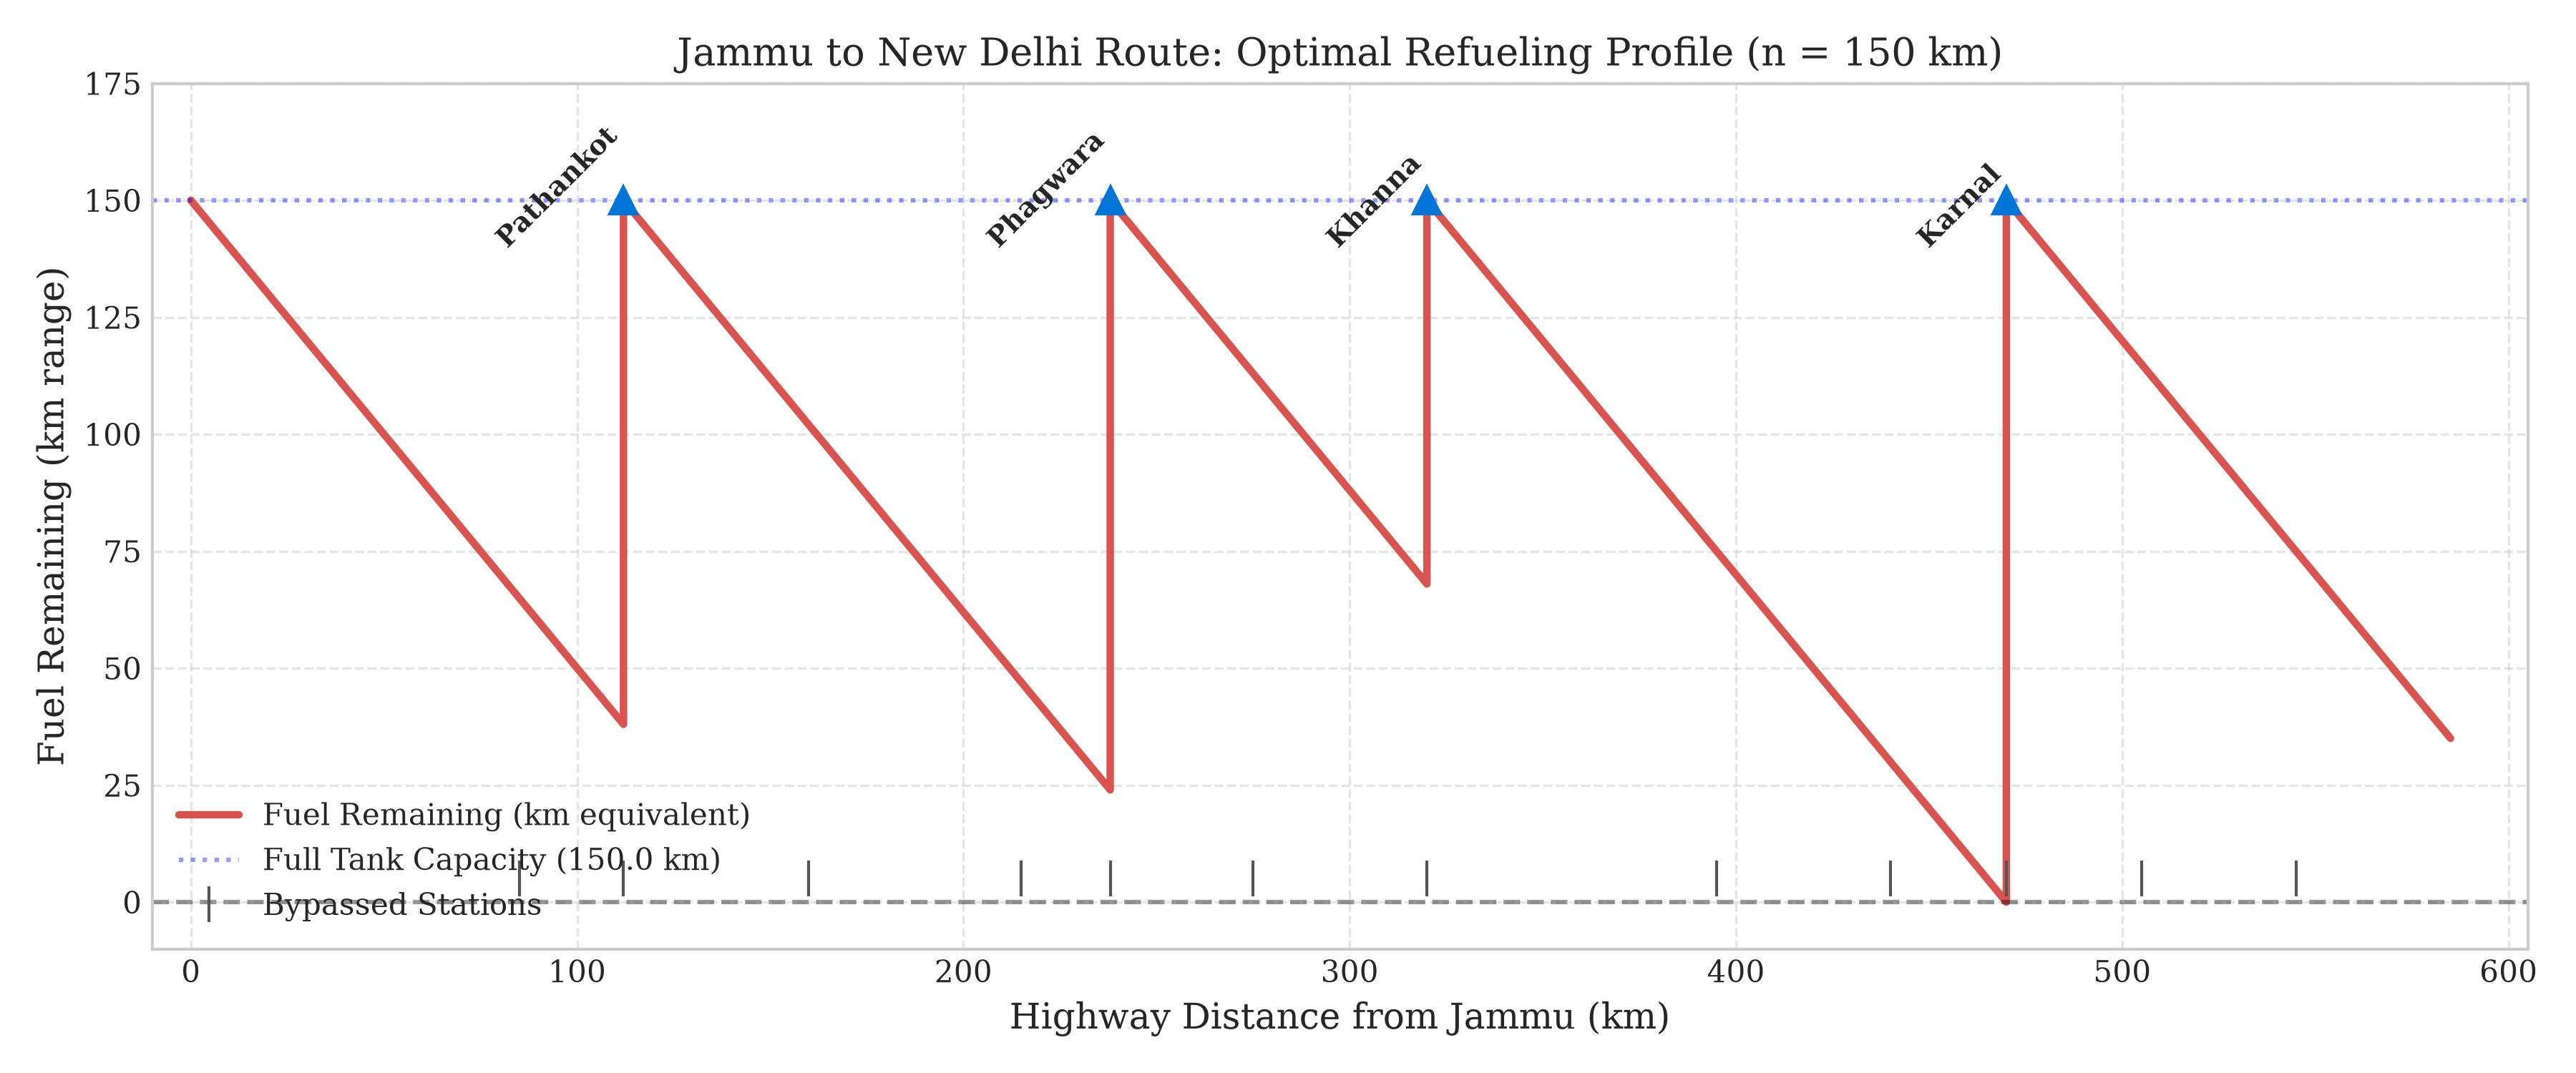
\includegraphics[width=0.92\textwidth]{images/petrol_stops_route_viz.png}
\caption{Refueling Profile from Jammu to New Delhi for Tank Capacity $n = 150\text{ km}$.}
\label{fig:petrol_stops}
\end{figure}

For $n = 150\text{ km}$, the algorithm selects exactly \textbf{4 stops}:
\begin{itemize}
    \item Stop 1: Pathankot Station ($112.0\text{ km}$ from Jammu)
    \item Stop 2: Phagwara Station ($238.0\text{ km}$ from Jammu, leg $= 126.0\text{ km}$)
    \item Stop 3: Khanna Station ($320.0\text{ km}$ from Jammu, leg $= 82.0\text{ km}$)
    \item Stop 4: Karnal Station ($470.0\text{ km}$ from Jammu, leg $= 150.0\text{ km}$)
    \item Final leg: Karnal to New Delhi ($115.0\text{ km}$ driven on last tank).
\end{itemize}

\newpage

% ==============================================================================
% ASSIGNMENT 9: BASE STATIONS
% ==============================================================================
\section*{Assignment 9: Cell Phone Base Station Placement on Country Road}

\subsection*{9.1 Problem Statement and Algorithmic Principle}
\textbf{Problem}: Houses are situated sparsely along a quiet country road at known distances $h_1, h_2, \dots, h_k$ from the western end. All residents utilize cell phones. Base stations (towers) have a coverage radius of $R = 4.0\text{ miles}$. Place the minimum number of towers such that every house is within $4\text{ miles}$ of at least one tower.

\textbf{Greedy Strategy}:
\begin{enumerate}
    \item Sort house locations: $h_1 \le h_2 \le \dots \le h_k$.
    \item Identify the leftmost uncovered house $h_i$.
    \item To cover $h_i$, a tower must be placed in $[h_i - R, h_i + R]$. To maximize rightward coverage for upcoming houses, place the tower as far east as possible:
    \[
    t = h_i + R
    \]
    \item This tower covers all houses in $[t - R, t + R] = [h_i, h_i + 2R]$.
    \item Skip all houses satisfying $h_j \le h_i + 2R$, and repeat for the next uncovered house.
\end{enumerate}

\textbf{Proof of Optimality}:
Any valid placement must cover the leftmost uncovered house $h_i$, requiring a tower at coordinate $t' \le h_i + R$. Our greedy placement sets $t^* = h_i + R \ge t'$. The interval covered to the right by $t^*$ is $[h_i, h_i + 2R]$, which is a superset of the rightward coverage $[t' - R, t' + R]$ of any $t' \le h_i + R$. Hence, choosing $t^*$ leaves fewer or equal remaining houses to cover. By induction, the greedy strategy achieves the minimal number of base stations.

\subsection*{9.2 Python Implementation (\texttt{base\_stations.py})}
\begin{lstlisting}[language=Python]
def place_base_stations(
    house_positions: List[float],
    coverage_radius: float = 4.0,
) -> Tuple[int, List[float], Dict[float, List[float]]]:
    if not house_positions:
        return 0, [], {}
    sorted_houses = sorted(house_positions)
    k = len(sorted_houses)
    station_locations = []
    coverage_map = {}
    idx = 0

    while idx < k:
        uncovered_house = sorted_houses[idx]
        tower_pos = uncovered_house + coverage_radius
        station_locations.append(tower_pos)
        coverage_map[tower_pos] = []

        max_reach = tower_pos + coverage_radius
        while idx < k and sorted_houses[idx] <= max_reach:
            coverage_map[tower_pos].append(sorted_houses[idx])
            idx += 1

    return len(station_locations), station_locations, coverage_map
\end{lstlisting}

\subsection*{9.3 Execution Visualization \& Verification}
\begin{figure}[H]
\centering
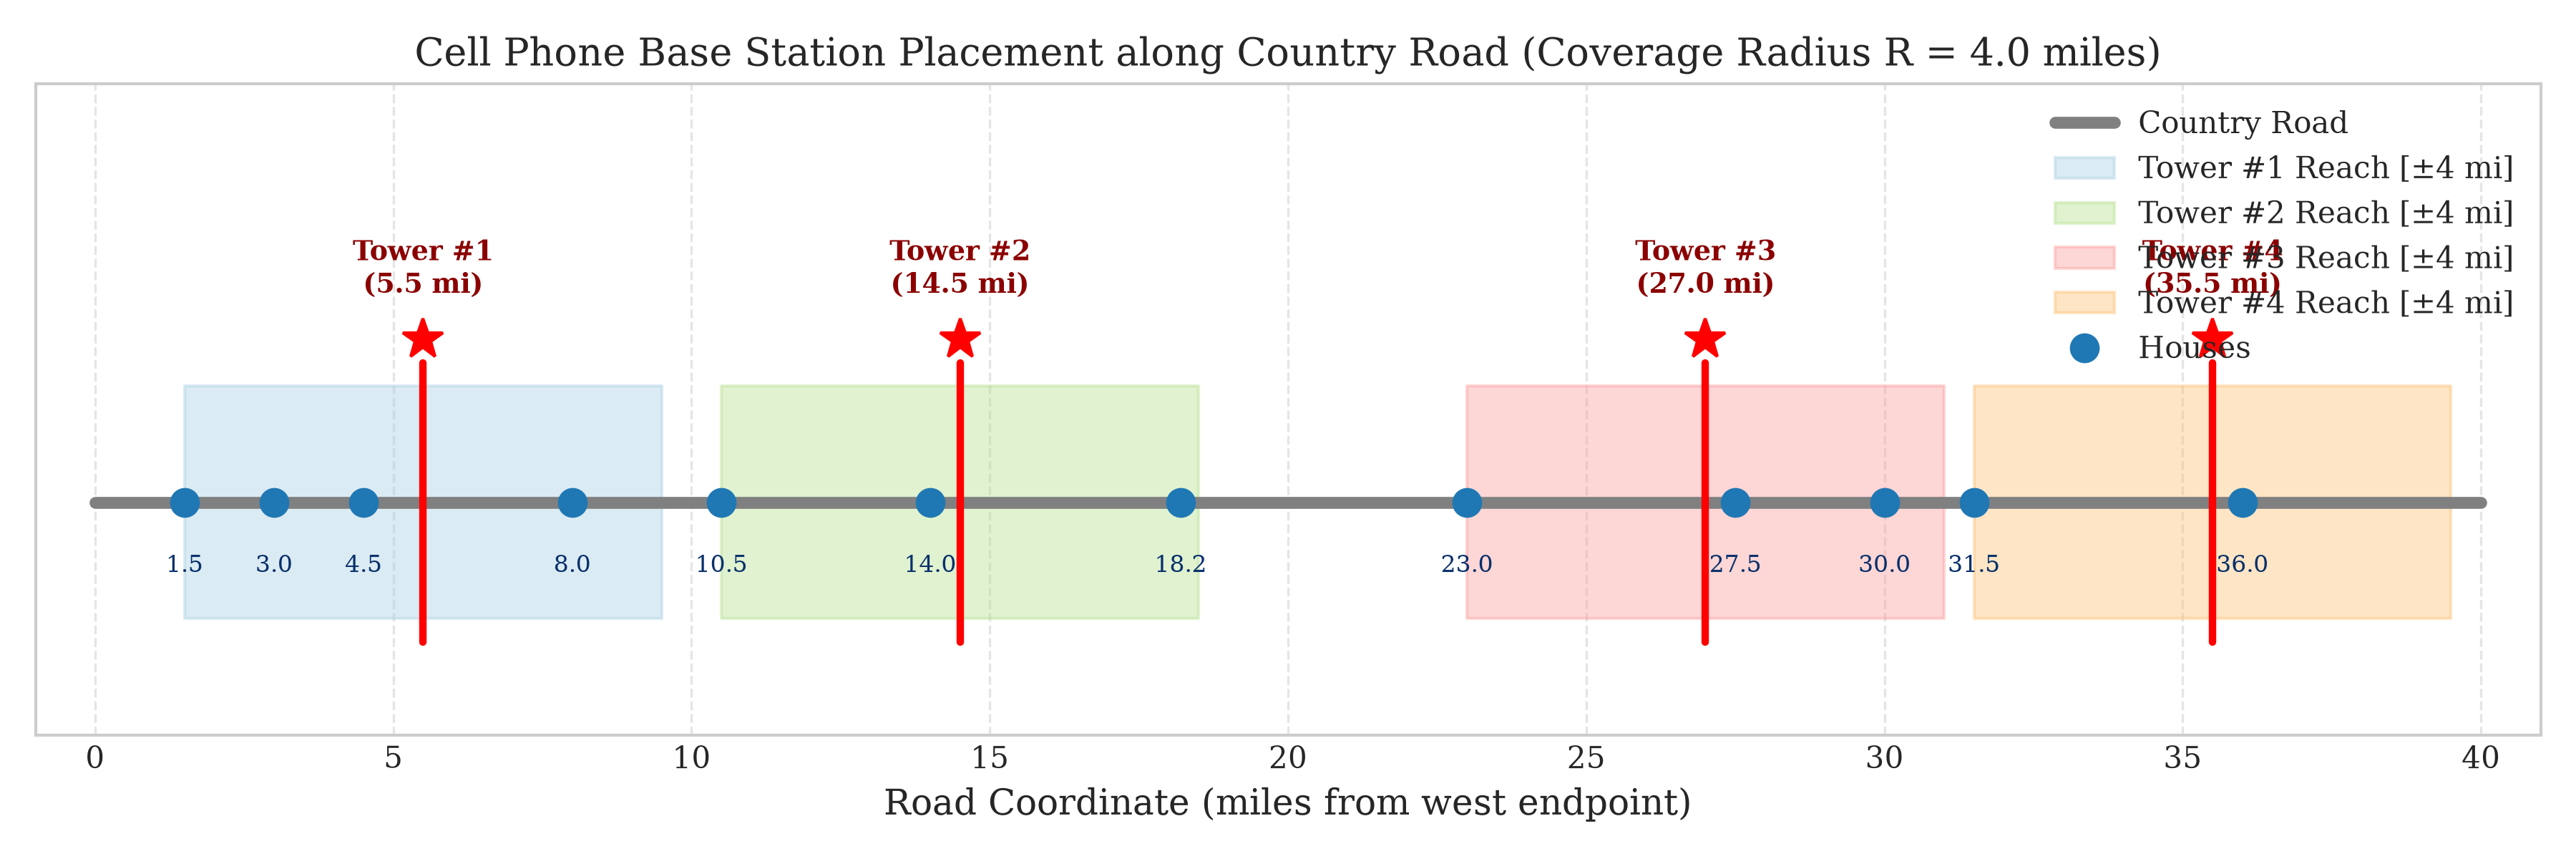
\includegraphics[width=0.92\textwidth]{images/base_station_coverage_viz.png}
\caption{Greedy Base Station Placement along Country Road: Towers at $5.5, 14.5, 27.0, 35.5\text{ miles}$.}
\label{fig:base_stations}
\end{figure}

For houses at $[1.5, 3.0, 4.5, 8.0, 10.5, 14.0, 18.2, 23.0, 27.5, 30.0, 31.5, 36.0]$ miles:
\begin{itemize}
    \item Tower 1 at mile $5.5$ (Coverage $[1.5 - 9.5]$): Covers houses at $\{1.5, 3.0, 4.5, 8.0\}$.
    \item Tower 2 at mile $14.5$ (Coverage $[10.5 - 18.5]$): Covers houses at $\{10.5, 14.0, 18.2\}$.
    \item Tower 3 at mile $27.0$ (Coverage $[23.0 - 31.0]$): Covers houses at $\{23.0, 27.5, 30.0\}$.
    \item Tower 4 at mile $35.5$ (Coverage $[31.5 - 39.5]$): Covers houses at $\{31.5, 36.0\}$.
\end{itemize}
All houses are strictly within $4.0\text{ miles}$ of an assigned tower. Minimum towers required: \textbf{4}.

\newpage

% ==============================================================================
% SYNTHESIS MATRIX & CONCLUSION
% ==============================================================================
\section*{Comprehensive Algorithmic Synthesis \& Comparison Matrix}

Table \ref{tab:comparison_all} synthesizes the core mathematical properties, algorithmic paradigms, time complexities, auxiliary memory requirements, and optimality guarantees across all nine lab assignments.

\begin{table}[H]
\centering
\caption{Synthesis of Algorithmic Paradigms, Complexities, and Optimality Guarantees.}
\label{tab:comparison_all}
\vspace{0.2cm}
\resizebox{\textwidth}{!}{
\begin{tabular}{lllccc}
\toprule
\textbf{Assignment} & \textbf{Problem Domain} & \textbf{Core Paradigm} & \textbf{Time Complexity} & \textbf{Aux Space} & \textbf{Optimality Guarantee} \\
\midrule
\textbf{Assignment 1} & Billboard Placement       & Dynamic Programming & $\mathcal{O}(n \log n)$ & $\mathcal{O}(n)$ & Exact (Optimal Substructure) \\
\textbf{Assignment 2} & Lecture Hall Scheduling   & Greedy (Min-Heap)   & $\mathcal{O}(n \log n)$ & $\mathcal{O}(n)$ & Exact (Interval Depth $d$) \\
\textbf{Assignment 3} & Activity Selection (Dual) & Greedy (EFT / LST)  & $\mathcal{O}(n \log n)$ & $\mathcal{O}(n)$ & Exact (Time-Reversal Duality) \\
\textbf{Assignment 4} & Huffman Coding            & Greedy (Min-Heap)   & $\mathcal{O}(N)$        & $\mathcal{O}(|\Sigma|)$ & Exact (Prefix-Free Tree Cost) \\
\textbf{Assignment 5} & Knapsack Equal Weights    & Quickselect         & $\mathcal{O}(m)$        & $\mathcal{O}(n)$ & Exact (Top-$k$ Profit Reduction) \\
\textbf{Assignment 6} & Knapsack Sorted Variant   & Greedy Scan         & $\mathcal{O}(n \log n)$ & $\mathcal{O}(n)$ & Exact (Exchange Argument) \\
\textbf{Assignment 7} & Knapsack Profit Order     & Greedy vs. DP       & $\mathcal{O}(n \log n)$ & $\mathcal{O}(n)$ & Unbounded Ratio $\frac{F^*(I)}{F(I)} \to \infty$ \\
\textbf{Assignment 8} & Refueling Stops           & Greedy Scan         & $\mathcal{O}(m \log m)$ & $\mathcal{O}(m)$ & Exact (Furthest Station Reach) \\
\textbf{Assignment 9} & Base Station Placement    & Greedy Scan         & $\mathcal{O}(k \log k)$ & $\mathcal{O}(k)$ & Exact (Max-Reach Shift Argument) \\
\bottomrule
\end{tabular}
}
\end{table}

\subsection*{Conclusion}
The algorithmic investigations conducted across Lab Assignment 8 yield several fundamental theoretical and practical insights:
\begin{enumerate}
    \item \textbf{When Greedy Solves NP-Hard Problems}: While general $0/1$ Knapsack is NP-hard, imposing structural constraints fundamentally collapses the problem complexity:
    \begin{itemize}
        \item When item weights are uniform ($w_i = w_0$), the problem reduces to top-$k$ order selection, solvable in $\mathcal{O}(m)$ time via Quickselect.
        \item When weights and values are monotonically ordered ($w_i \uparrow \iff v_i \downarrow$), a greedy prefix scan provably delivers the exact optimal solution.
    \end{itemize}
    \item \textbf{The Peril of Flawed Greedy Heuristics}: Sorting knapsack items by profit value alone yields an unbounded approximation ratio ($\frac{F^*(I)}{F(I)} = R$ for arbitrary $R$), demonstrating that greedy heuristics ignoring resource costs can fail arbitrarily badly.
    \item \textbf{Exchange Arguments as Universal Proof Mechanisms}: Interval scheduling, lecture hall partitioning, petrol refueling, and base station placement are all rigorously validated through exchange arguments, showing that local choices never preclude a globally optimal configuration.
\end{enumerate}

\end{document}
